
% ----------------------------------------------------------------------
%  Set the document class
% ----------------------------------------------------------------------
\documentclass[11pt,a4paper,twoside]{article}

% ----------------------------------------------------------------------
% Define external packages, language, margins, fonts and new commands
% ----------------------------------------------------------------------
%\input{preamble} 
\usepackage[utf8]{inputenc}   % <<<<< Linux
\usepackage[english]{babel} % <<<<< English
\usepackage{notoccite}
\usepackage[skip=0.5\baselineskip]{caption}
\hyphenation{GTKWave}
\usepackage{listings}
\usepackage{amsmath}
\usepackage[all]{nowidow}

%blind text

\usepackage{graphicx}
\graphicspath{{./}{../../figlib/}{../mat/}{../sim/}}
\def\FontLn{% 16 pt normal
  \usefont{T1}{phv}{m}{n}\fontsize{16pt}{16pt}\selectfont}
\def\FontLb{% 16 pt bold
  \usefont{T1}{phv}{b}{n}\fontsize{16pt}{16pt}\selectfont}
\def\FontMn{% 14 pt normal
  \usefont{T1}{phv}{m}{n}\fontsize{14pt}{14pt}\selectfont}
\def\FontMb{% 14 pt bold
  \usefont{T1}{phv}{b}{n}\fontsize{14pt}{14pt}\selectfont}
\def\FontSn{% 12 pt normal
  \usefont{T1}{phv}{m}{n}\fontsize{12pt}{12pt}\selectfont}

% Use Arial font as default
%
\renewcommand{\rmdefault}{phv}
\renewcommand{\sfdefault}{phv}
\usepackage{geometry}	
\geometry{verbose,tmargin=2.5cm,bmargin=2.5cm,lmargin=2.5cm,rmargin=2.5cm}

%\usepackage{setspace}
%\renewcommand{\baselinestretch}{1.5}

\usepackage[pdftex]{hyperref} % enhance documents that are to be
                              % output as HTML and PDF
\hypersetup{colorlinks,       % color text of links and anchors,
                              % eliminates borders around links
%            linkcolor=red,    % color for normal internal links
            linkcolor=black,  % color for normal internal links
            anchorcolor=black,% color for anchor text
%            citecolor=green,  % color for bibliographical citations
            citecolor=black,  % color for bibliographical citations
%            filecolor=magenta,% color for URLs which open local files
            filecolor=black,  % color for URLs which open local files
%            menucolor=red,    % color for Acrobat menu items
            menucolor=black,  % color for Acrobat menu items
%            pagecolor=red,    % color for links to other pages
            pagecolor=black,  % color for links to other pages
%            urlcolor=cyan,    % color for linked URLs
            urlcolor=black,   % color for linked URLs
	          bookmarks=true,         % create PDF bookmarks
	          bookmarksopen=false,    % don't expand bookmarks
	          bookmarksnumbered=true, % number bookmarks
	          pdftitle={report},
            pdfauthor={Andre C. Marta},
%            pdfsubject={Thesis Title},
%            pdfkeywords={Thesis Keywords},
            pdfstartview=FitV,
            pdfdisplaydoctitle=true}

\usepackage[numbers,sort&compress]{natbib} % <<<<< References in numbered list [1],[2],...
\usepackage{subcaption} 
\usepackage{mdframed}

%%%%%%%%%%%%%%%%%%%%%%%%%%%%%%%%%%%%%%%%%%%%%%%%%%%%%%%%%%%%%%%%%%%%%%%%
%     Begin Document                                                   %
%%%%%%%%%%%%%%%%%%%%%%%%%%%%%%%%%%%%%%%%%%%%%%%%%%%%%%%%%%%%%%%%%%%%%%%%


\begin{document}

% Set plain page style (no headers, footer with centered page number)
\pagestyle{plain}

% Set roman numbering (i,ii,...) before the start of chapters
%\pagenumbering{roman}

% ----------------------------------------------------------------------
%  Cover page
% ----------------------------------------------------------------------
%%%%%%%%%%%%%%%%%%%%%%%%%%%%%%%%%%%%%%%%%%%%%%%%%%%%%%%%%%%%%%%%%%%%%%%%
%                                                                      %
%     File: Thesis_FrontCover.tex                                      %
%     Tex Master: Thesis.tex                                           %
%                                                                      %
%     Author: Andre C. Marta                                           %
%     Last modified :  2 Jul 2015                                      %
%                                                                      %
%%%%%%%%%%%%%%%%%%%%%%%%%%%%%%%%%%%%%%%%%%%%%%%%%%%%%%%%%%%%%%%%%%%%%%%%

\thispagestyle {empty}

% IST Logo - Signature A
% parameters: bb=llx lly urx ury (bounding box), width=h_length, height=v_length, angle=angle, scale=factor, clip=true/false, draft=true/false. 

\includegraphics[bb=9.5cm 11cm 0cm 0cm,scale=0.29]{IST_A_CMYK_POS}

\begin{center}
%
% Figure (Image or plot)
\vspace{1.0cm}
% height = 50 mm
%\includegraphics[height=50mm]{Figures/Airbus_A350.jpg}

% Title, author and degree
\vspace{1cm}
{\FontLb Lab 02 Report} \\ % <<<<< EDIT TITLE
{\FontSn Circuit Theory and Eletronic's Fundamentals} \\ % <<<<< EDIT COURSE
\vspace{1cm}
{\FontSn Afonso Guerreiro (96501) Diogo Aguiar (96520) Francisco Raposo (96531) \\Instituto Superior Técnico\\ Mestrado em Engenharia Física Tecnológica\\}
\vspace{1cm}
{\FontSn March 23, 2021} \\ % <<<<< EDIT DATE (corresponds to date of oral examination)
%
\end{center}



% ----------------------------------------------------------------------
% Dedication page (optional)
% ----------------------------------------------------------------------
%\input{dedication} 
%\cleardoublepage

% ----------------------------------------------------------------------
%  Acknowledgments (optional)
% ----------------------------------------------------------------------
%\input{acknowledgements}
%\cleardoublepage

% ----------------------------------------------------------------------
%  Abstract (both in English and Portuguese)
% ----------------------------------------------------------------------
%\input{resumo} 
%\cleardoublepage

%\input{abstract} 

% ----------------------------------------------------------------------
%  Table of contents, list of tables, list of figures and nomenclature
% ----------------------------------------------------------------------

% Table of contents
%
\tableofcontents

% List of tables
%\addcontentsline{toc}{section}{\listtablename}
%\listoftables
%\cleardoublepage 

% List of figures
%\addcontentsline{toc}{section}{\listfigurename}
%\listoffigures
%\cleardoublepage 

% Set arabic numbering (1,2,...) after preface
%
%\setcounter{page}{1}
%\pagenumbering{arabic}

% ----------------------------------------------------------------------
%  Body
% ----------------------------------------------------------------------

\section{Introduction}
\label{sec:introduction}

% state the learning objective 
The objective of this laboratory assignment is to study a circuit containing a
sinusoidal voltage source $V_I$ connected to a resistor $R$ and a capacitor $C$
in series. The circuit can be seen if Figure~\ref{fig:rc}.

\lipsum[1-1]

In Section~\ref{sec:analysis}, a theoretical analysis of the circuit is
presented. In Section~\ref{sec:simulation}, the circuit is analysed by
simulation and the results are compared to the theoretical results obtained in
Section~\ref{sec:analysis}. The conclusions of this study are oulined in
Section~\ref{sec:conclusion}.

\begin{figure}[h] \centering
\includegraphics[width=0.4\linewidth]{rc.pdf}
\caption{Voltage driven serial RC circuit.}
\label{fig:rc}
\end{figure}



\section{Theoretical Analysis}
\label{sec:analysis}

In this section, the circuit shown in Figure~\ref{fig:rc} is analysed
theoretically, in terms of its time and frequency responses.

\section{Time response}

The circuit consists of a single V-R-C loop where a current $i(t)$ circulates. The
voltage source $v_I(t)$ drives its input, and the output voltage $v_O(t)$ is taken from
the capacitor terminals. Applying the Kirchhoff Voltage Law (KVL), a single
equation for the single loop in the circuit can be written as

\begin{equation}
  Ri(t) + v_O(t) = v_I(t).
  \label{eq:kvl}
\end{equation}

Because $v_O$ is the voltage between capacitor C's plates, it is related to the
current $i$ by
\begin{equation}
  i(t) = C\frac{dv_O}{dt}.
\end{equation}

Hence, Equation~(\ref{eq:kvl}) can be rewritten as
\begin{equation}
  RC\frac{dv_O}{dt} + v_O(t) = v_I.
  \label{eq:kvl2}
\end{equation}

Equation~(\ref{eq:kvl2}) is a linear differencial equation whose solution is a
superposition of a natural solution $v_{On}$ and a forced solution $v_{Of}$:

\begin{equation}
  v_O(t) = v_{On}(t) + v_{Of}(t).
  \label{eq:vo_sol}
\end{equation}

As learned in the theory classes the natural solution is of the form
\begin{equation}
  v_{On}(t) = Ae^{-\frac{t}{RC}},
  \label{eq:vo_nat}
\end{equation}
where $A$ is an integration constant.

The forced solution is of the form given in Equation~(\ref{eq:vo_for}) and is
illustrated in Figure~\ref{fig:forced}.

\begin{equation}
  V_{Of}(t) = |\bar{V}_{Of}| cos(\omega t + \angle \bar{V}_{Of}),
  \label{eq:vo_for}
\end{equation}

\lipsum[1-1]


\begin{figure}[h] \centering
\includegraphics[width=0.8\linewidth]{forced.eps}
\caption{Forced sinusoidal response.}
\label{fig:forced}
\end{figure}

\section{Frequency response}

\lipsum[1-1]




\section{Simulation Analysis}

Using the ngspice program, we began by analysing the circuit for $t<0$, the currents and voltages at each node are summarized in the table below.

%%%%%INCLUDE TABLE 
\begin{table}[h]
  \centering
  \begin{tabular}{|l|r|}
    \hline    
    {\bf Name} & {\bf Value [A or V]} \\ \hline
    @r1[i] & -2.58478e-04\\ \hline
@r2[i] & 2.705006e-04\\ \hline
@r3[i] & -1.20225e-05\\ \hline
@r4[i] & -1.17739e-03\\ \hline
@r5[i] & 2.705006e-04\\ \hline
@r6[i] & 9.189098e-04\\ \hline
@r7[i] & 9.189098e-04\\ \hline
@c[i] & 0.000000e+00\\ \hline
v(1) & 5.134559e+00\\ \hline
v(2) & 4.871563e+00\\ \hline
v(3) & 4.321260e+00\\ \hline
v(4) & -1.87652e+00\\ \hline
v(5) & 4.908647e+00\\ \hline
v(6) & 5.722227e+00\\ \hline
v(7) & -1.87652e+00\\ \hline
v(8) & -2.80082e+00\\ \hline

  \end{tabular}
  \caption{Operating point. A variable preceded by @ is of type {\em current}
    and expressed in mA; other variables are of type {\it voltage} and expressed in
    Volt.}
  \label{tab:op1}
\end{table}

Then we proceeded to calculate the tensions $V_6$ and $V_8$, for time $t=0s$, with an applied tension of $0V$, and where the capacitor was substituted by a independent voltage source which imposes a voltage equal to $V_6-V_8$. This is indeed, necessary to establish the boundary conditions for the system, for $t>0s$, since in the instant $t=0s$ the applied tension is $0v$, thus by performing the operating point analyses for the conditions described above, the initial values of the aforementioned tensions may be obtained. The capacitor is replaced by a voltage source because at that instant for our purposes the tension at each of its terminals is constant since we are holding time still.
The results that were obtained are shown bellow


%%%%%INCLUDE TABLE 
\begin{table}[h]
  \centering
  \begin{tabular}{|l|r|}
    \hline    
    {\bf Name} & {\bf Value [A or V]} \\ \hline
    @r1[i] & -2.58478e-04\\ \hline
@r2[i] & 2.705006e-04\\ \hline
@r3[i] & -1.20225e-05\\ \hline
@r4[i] & -1.17739e-03\\ \hline
@r5[i] & 2.705006e-04\\ \hline
@r6[i] & 9.189098e-04\\ \hline
@r7[i] & 9.189098e-04\\ \hline
@c[i] & 0.000000e+00\\ \hline
v(1) & 5.134559e+00\\ \hline
v(2) & 4.871563e+00\\ \hline
v(3) & 4.321260e+00\\ \hline
v(4) & -1.87652e+00\\ \hline
v(5) & 4.908647e+00\\ \hline
v(6) & 5.722227e+00\\ \hline
v(7) & -1.87652e+00\\ \hline
v(8) & -2.80082e+00\\ \hline

  \end{tabular}
  \caption{Operating point for $V_s = 0$V and  $t = 0$s. A variable preceded by @ is of type {\em current}
    and expressed in mA; other variables are of type {\it voltage} and expressed in
    Volt.}
  \label{tab:op1}
\end{table}


Using the results listed above, we then simulated the natural response of the circuit, imposing that the initial voltage at node 6 be equal to what we obtained beforehand. To accomplish it, we set the independent voltage source to $0V$ and ,as was expected, the capacitor discharged, following a negative exponential model, as is shown 

%%%%%INCLUDE BONECO DA SOLUÇÃO NATURAL
\begin{figure}[h] \centering
\includegraphics[width=0.6\linewidth]{../sim/3/trans.pdf}
\caption{Natural solution for $t > 0$ s}
\label{fig:Natural solution}
\end{figure}

We then, repeated the same process but this time for the general solution, consisting on the natural and the forced solutions, with the same initial conditions as before. We expected to observe a sinusoidal signal of the same frequency of the applied tension, supper imposed with the previous exponential solution, which as we can see was obtained 


%%%%%INCLUDE BONECO DA SOLUÇÃO GERAL
\begin{figure}[h] \centering
\includegraphics[width=0.6\linewidth]{../sim/4/trans.pdf}
\caption{Full solution for $t > 0$ s}
\label{fig:Full solution}
\end{figure}

At last, we simulated the systems response to several different driving frequencies ranging from 0.1Hz to 1MHz, and the resultant magnitude and phase of the ensuing voltages ($V_6,V_S,V_C$) where plotted, the first the magnitude was expressed in decibels, the second in degrees, and in both cases the x scale is logarithmic. The graphs obtained follow


%%%%%INCLUDE BONECO DA FASE E ÂNGULO
\begin{figure}[h] \centering
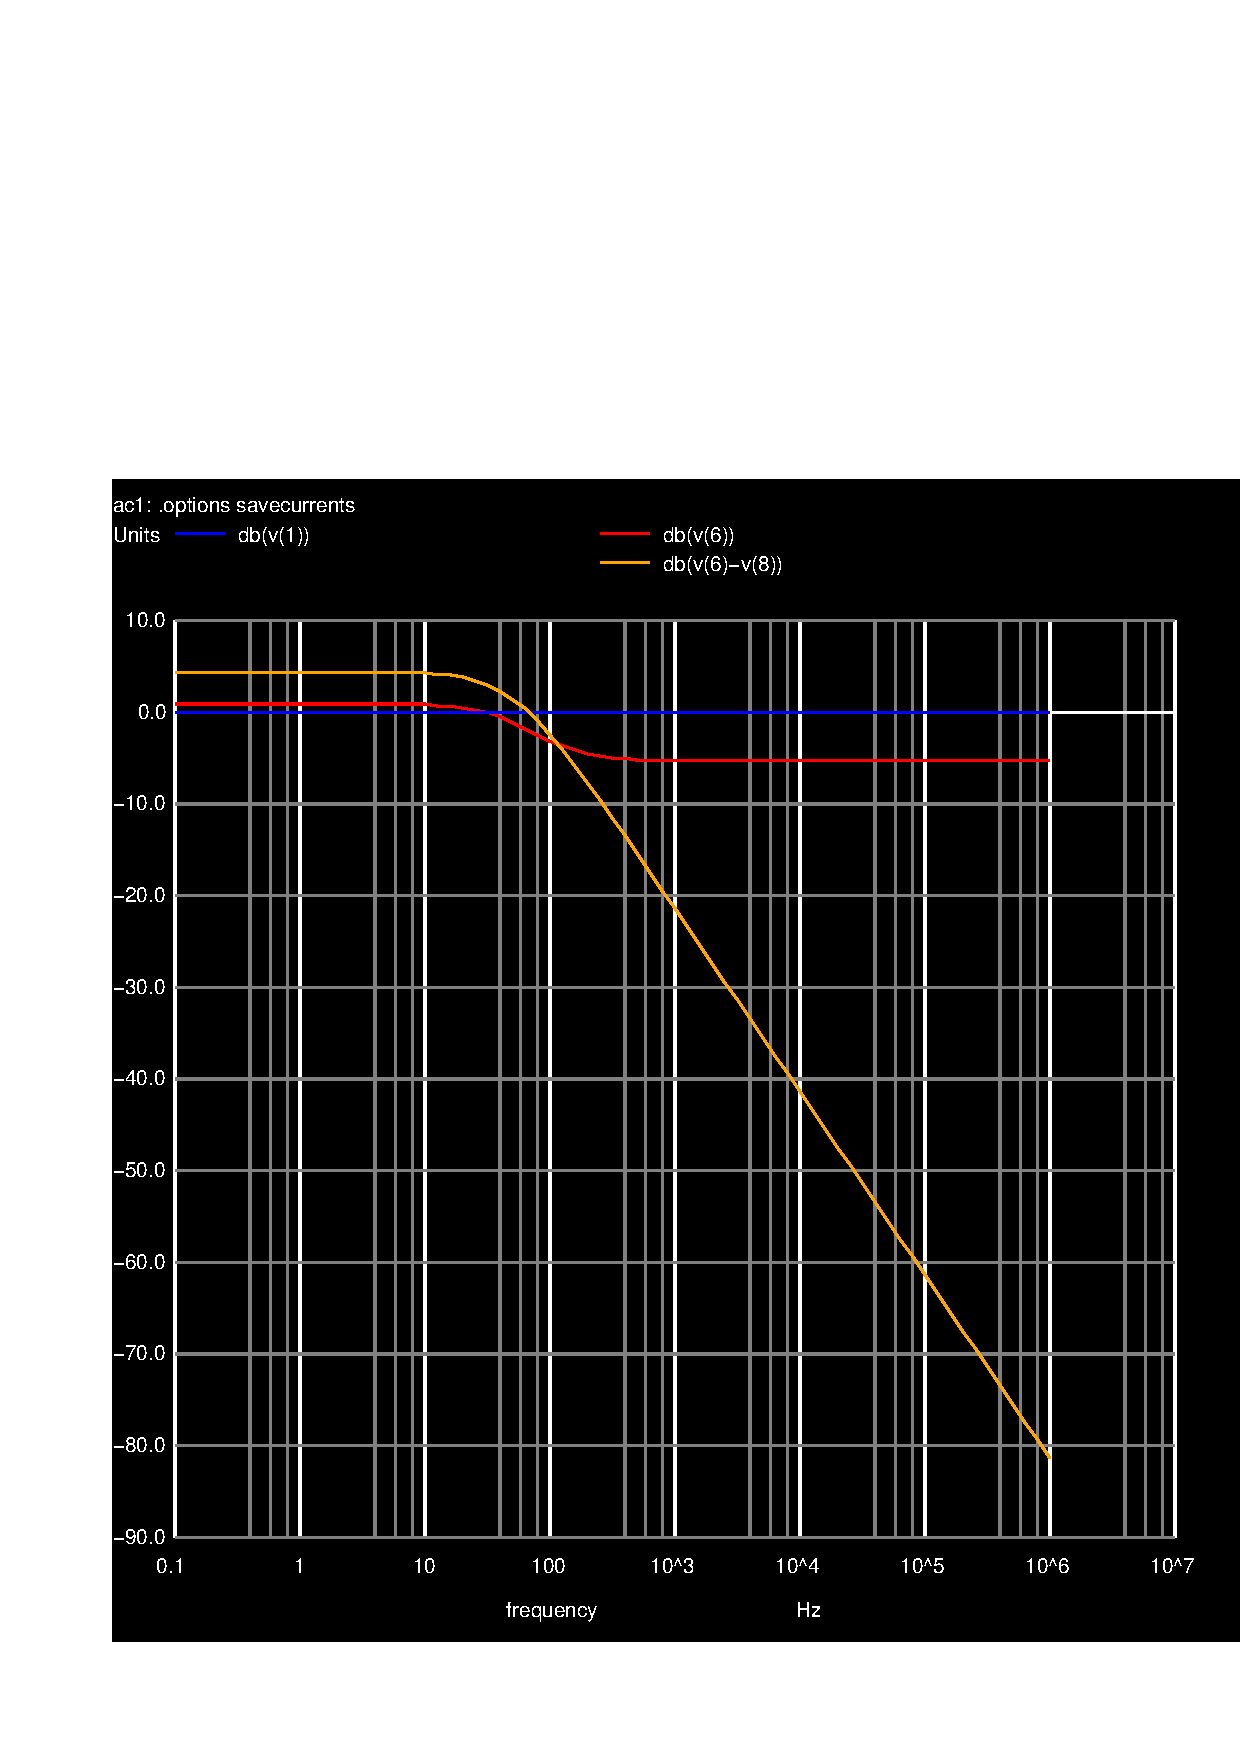
\includegraphics[width=0.6\linewidth]{../sim/5/acm.pdf}
\caption{Circuit's amplitude response}
\label{fig:Amp response}
\end{figure}

\begin{figure}[h] \centering
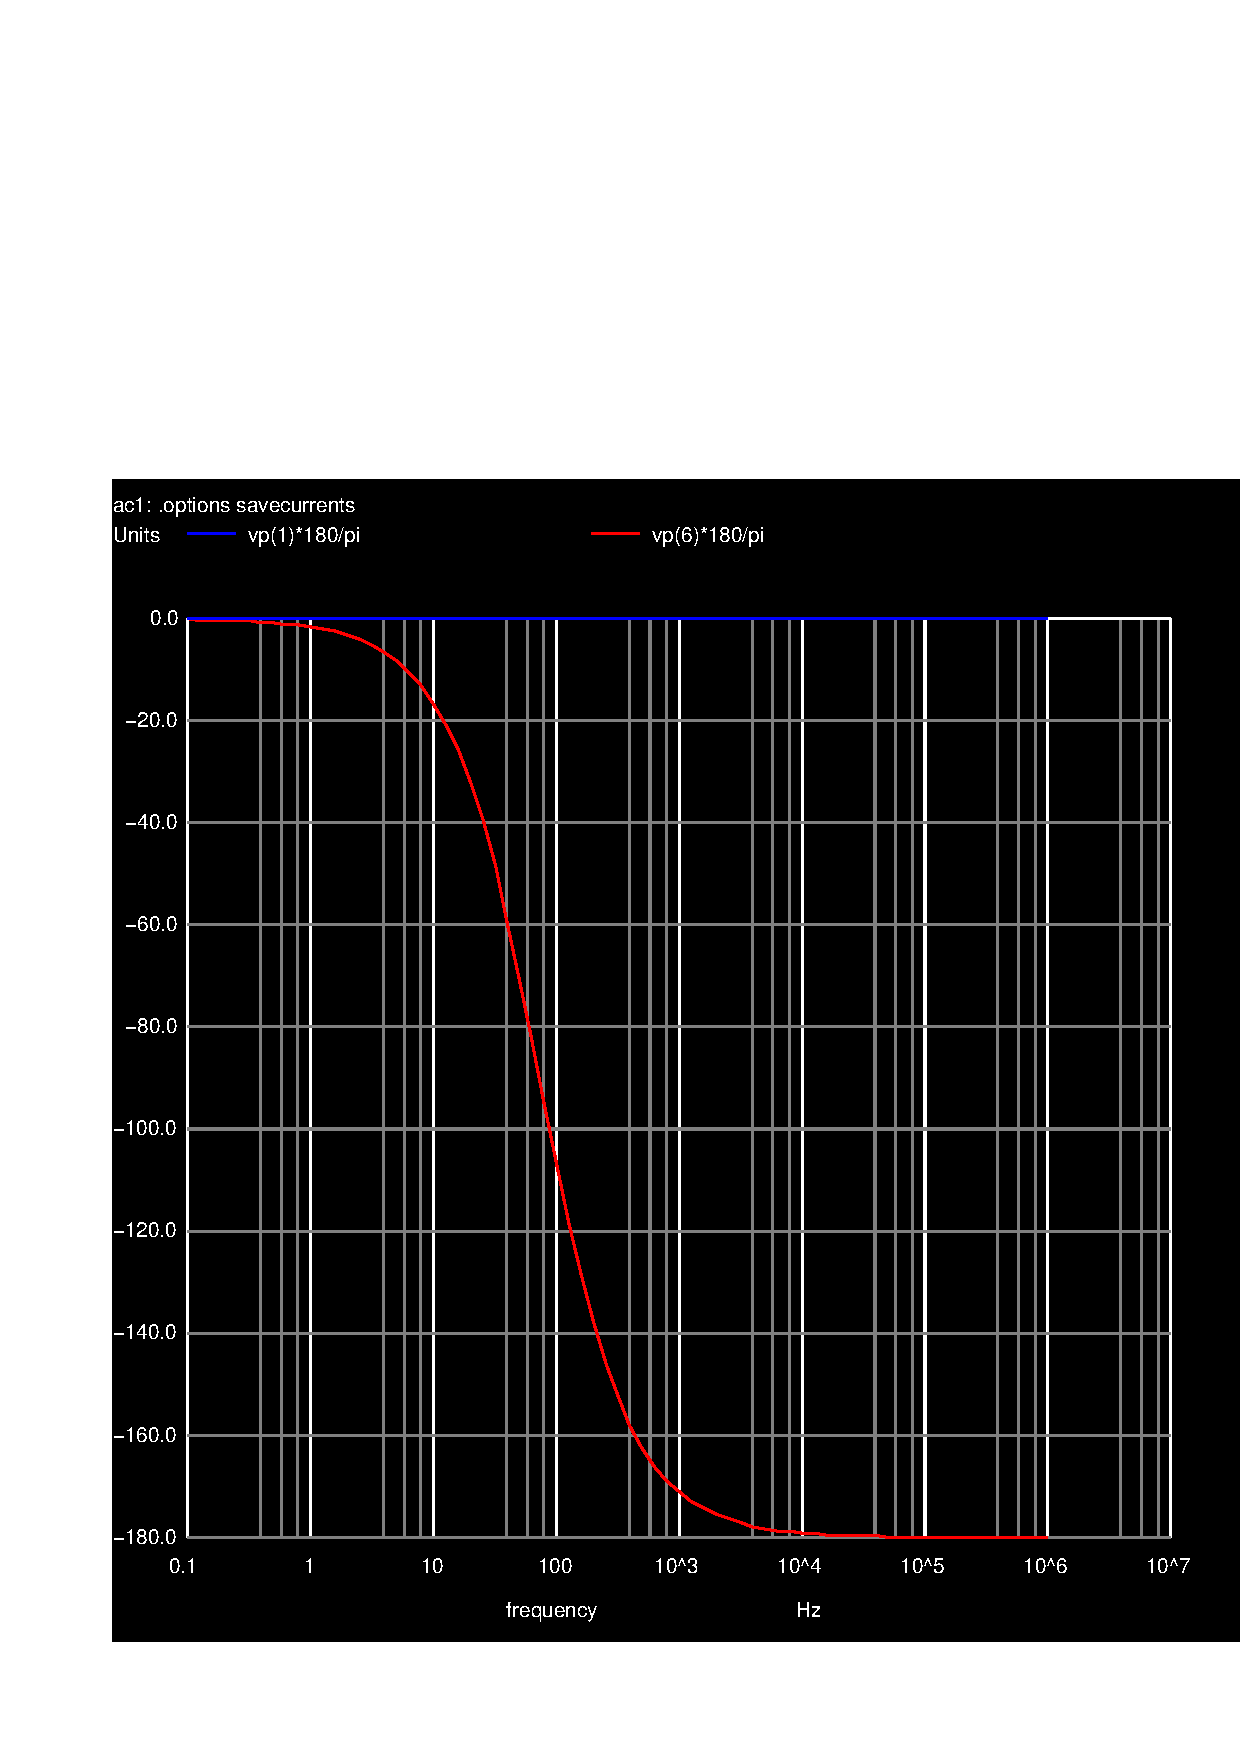
\includegraphics[width=0.6\linewidth]{../sim/5/freq.pdf}
\caption{Circuit's phase response}
\label{fig:Phase response}
\end{figure}









\section{Conclusion}
\label{sec:conclusion}

With this paper, we were able to see how the capacitor behaves when a constant voltage is supplied ans well as time varying, in the matter at hand, a sinusoidal signal. As we stated before the theoretical predictions made, were in close agreement with the simulation results obtained. Any differences obtained may be attributed to numerical errors or approximations committed while carrying out the maths, since this deviations were never greater than $1\%$ of the results obtained analytically. 
As stated before, the operating point analysis supported the results attained using nodal analysis. The simulated natural response closely resembled the exponential solution derived from first principles, and so did the general solution as we saw from the resemblance of both graphs. At last, the transfer function derived in the last section, was a close match to the plot obtained from \textit{ngspice}, allowing us to verify that high frequencies tend to have significantly lower voltage magnitudes than lower frequencies at the terminals of the capacitor, thus as said before the system behaves as low pass filter.

%\cleardoublepage

% ----------------------------------------------------------------------
%  Bibliography
% ----------------------------------------------------------------------
%\addcontentsline{toc}{section}{\bibname}
%\bibliographystyle{abbrvunsrtnat} % <<<<< SELECT IF USING REFERENCES BY NUMBER (CITATION ORDER)
%\bibliography{../../../BIBfile.bib}

% ----------------------------------------------------------------------
\end{document}
% ----------------------------------------------------------------------
